\chapter{Sorrow, Passion, and Beauty}

This chapter follows J. Krishnamurti's dialogue with Dr. Alan W. Anderson on sorrow, passion, beauty, and action. The source is the Krishnamurti Foundation Trust material for the San Diego 1974 conversations, curated here by LazyingArt LLC through the Video2Book course workflow. There is no blackboard in this lecture, and no validated screenshot is useful for mathematical reconstruction. The structure below is therefore a careful conceptual calculus: we keep the order of the spoken inquiry while using compact equations and diagrams only as notation for distinctions Krishnamurti actually makes.

\section{From Beauty as Object to Beauty as Inquiry}

Anderson begins by placing this conversation in the path of the previous inquiry. They had been speaking about fear, transformation, knowledge, time, and pleasure. At the end of that discussion the question of beauty appeared. That matters, because beauty is not introduced here as an ornament or as a cultural topic. It is a test case for the whole inquiry into freedom. If transformation is not dependent on knowledge and time, then beauty cannot be merely what knowledge has told us to admire.

Krishnamurti begins with museums. Why are they so full of pictures and statues? Is it because human beings have lost touch with nature and therefore go to look at other people's expressions of beauty? He is not saying that museums should or should not exist. He is asking why we look outward so quickly, why we defer to paintings, poems, cathedrals, experts, and guided tours.

So the first distinction is not between beautiful and ugly objects. It is between direct inquiry and second-hand recognition. We can write this, cautiously, as

\begin{equation}
\text{beauty as object} \neq \text{the inquiry into beauty}.
\end{equation}

The inequality is not a formal theorem. It is a reminder. A painting, a poem, a cathedral, or a word may express something; but the expression is not the same as the seeing of beauty. The danger is that we begin with the museum and never ask what quality of mind is capable of beauty.

\begin{remark}
The lecture does not reject art. It rejects the assumption that accumulated judgment about art is the same thing as beauty. The chapter should preserve that delicacy.
\end{remark}

This is why Krishnamurti's first question has to remain open: must beauty be expressed? Does it need stone, colour, paint, word, or building? Or is there something which cannot be reduced to those forms? He does not answer immediately. He turns the inquiry inward, and the next word is not aesthetics but suffering.

\section{Sorrow, Passion, and the Humility of Not Knowing}

Krishnamurti's first major pivot is sharp: to inquire into beauty deeply, one must understand suffering. Without passion, he says, there is no beauty; but passion is not lust, and not the cultivated intensity of trying to be passionate. It is connected with the mind that remains with suffering and does not escape.

A compact form of the lecture's first chain is

\begin{equation}
\text{sorrow}
\xrightarrow{\text{non-withdrawal}}
\text{passion}
\xrightarrow{\text{sensitivity}}
\text{beauty}.
\end{equation}

This is a transcript-based schematic, not a psychological law. Its value is that it keeps the order of the inquiry visible. Beauty is not reached by appreciation alone. It depends on sensitivity. Sensitivity depends here on passion. Passion is born, not manufactured, when sorrow is neither avoided nor explained away.

Krishnamurti then corrects the speed of his own movement. Anderson hears the link between sorrow and beauty and begins to clarify: not that one must suffer. Krishnamurti agrees in effect and says they must go more slowly. The mind assumes it knows what beauty is. It has learned names, schools, painters, cathedrals, guided tours, expert accounts. But if one is really inquiring, one begins with humility: I do not know.

\subsection{Question \& Answer}

\paragraph{Question.}
Does the connection between sorrow, passion, and beauty mean that suffering is required, or that suffering should be cultivated?

\paragraph{Answer.}
No. Krishnamurti explicitly slows the inquiry at this point. The point is not that one must suffer, nor that suffering has value as an ideal. The point is that the mind usually escapes from sorrow, and therefore never understands it. Beauty cannot be approached by forcing sorrow, but neither can it be approached by running away from sorrow.

The working distinction is

\begin{align}
\text{cultivated suffering} &\neq \text{understanding sorrow},\\
\text{cultivated passion} &\neq \text{passion born from non-withdrawal}.
\end{align}

The proper beginning is not effort, belief, or method, but not-knowing. That very not-knowing is already part of the beauty Krishnamurti is pointing toward.

\section{The Movement Away from Sorrow}

Krishnamurti next widens the field. There is personal sorrow, but there is also the sorrow of humanity: war, hunger, tyranny, loneliness, cruelty, poverty, the ordinary griefs of human beings. If one remains only with one's own sorrow, the immensity of human sorrow is missed. Yet the pattern of escape is similar.

In one culture sorrow may be delegated to a sacred figure. In another it may be rationalized through karma. Elsewhere it is escaped through drink, sex, ritual, entertainment, belief, identification with something larger than oneself, or a thousand private movements of comfort. The common structure is simple:

\begin{equation}
\text{what is}
\longrightarrow
\text{movement away}
\longrightarrow
\text{dissipation of energy}
\longrightarrow
\text{failure to understand what is}.
\end{equation}

Here ``what is'' is sorrow. The phrase does not mean a doctrine of reality in general. It names the actual fact in front of the mind. Any movement away from that fact consumes energy in escape, and that very movement prevents understanding.

\begin{figure}
\centering
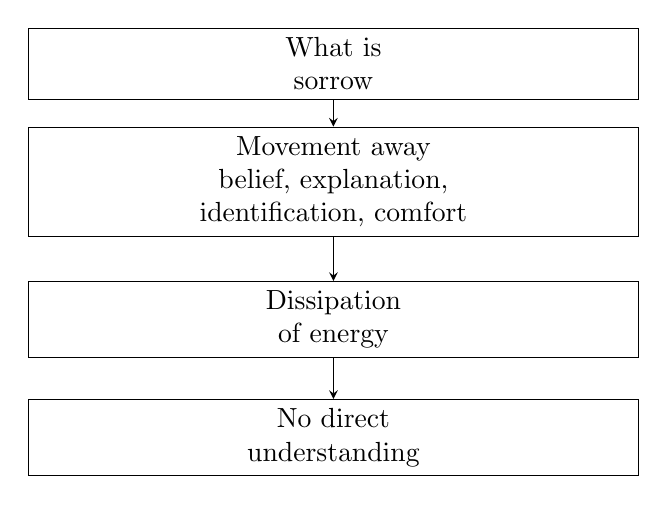
\begin{tikzpicture}[>=stealth]
\node[draw, align=center, text width=0.62\linewidth] (a) at (0,0) {What is\\sorrow};
\node[draw, align=center, text width=0.62\linewidth] (b) at (0,-1.5) {Movement away\\belief, explanation,\\identification, comfort};
\node[draw, align=center, text width=0.62\linewidth] (c) at (0,-3.25) {Dissipation\\of energy};
\node[draw, align=center, text width=0.62\linewidth] (d) at (0,-4.75) {No direct\\understanding};
\draw[->] (a) -- (b);
\draw[->] (b) -- (c);
\draw[->] (c) -- (d);
\end{tikzpicture}
\caption{Transcript-based schematic of escape from sorrow. The diagram is a conceptual reconstruction, not a blackboard figure.}
\end{figure}

This is one of the central movements of the lecture. Krishnamurti is not ranking escapes morally. He is showing that all escape has the same functional form: it moves away from the fact. The religious explanation, the philosophical explanation, the drink, the ritual, and the respectable belief may look different, but each may prevent the mind from remaining with sorrow.

\section{Non-Withdrawal and the Birth of Passion}

The next step is the lecture's first payoff. If the mind does not escape, rationalize, go beyond, or become frightened of sorrow, then it remains with it. Krishnamurti gives ordinary examples: an incident, a word, an accident, a shattering loneliness. Such events bring sorrow. The question is whether the mind can remain there without movement away.

We can make the contrast precise:

\begin{align}
E &= \text{escape from sorrow},\\
N &= \text{non-withdrawal from sorrow},\\
P &= \text{passion}.
\end{align}

The lecture does not state a formula, but its local logic is

\begin{align}
E &\Rightarrow \text{dissipated energy},\\
N &\Rightarrow P.
\end{align}

The second implication must be read cautiously. It is not a technique: perform non-withdrawal and obtain passion. Rather, when the mind is no longer scattering itself in escape, Krishnamurti says that passion is born. This passion is not artificial, not cultivated, not the result of trying to become passionate.

\subsection{Question \& Answer}

\paragraph{Question.}
What happens when sorrow is not consoled, explained, or escaped?

\paragraph{Answer.}
The ordinary assumption is that sorrow must be consoled. Anderson brings out the word ``disconsolate,'' and notes the usual movement: get rid of the lack of consolation. Krishnamurti's answer reverses the reflex. If there is no escape, no desire to seek comfort away from what is, then out of that reality comes passion.

The useful note-form is

\begin{equation}
\text{no escape} + \text{remaining with sorrow}
\;\longrightarrow\;
\text{passion}.
\end{equation}

This is also why beauty is not merely the appreciation of a painting, poem, or statue. Without the inward quality of passion, beauty remains second-hand or intellectual.

\begin{remark}
The word ``passion'' should not be allowed to drift into excitement, enthusiasm, or emotional intensity. In this lecture it is tied to sorrow, non-withdrawal, abandonment of the self, and austerity in the sense of inward simplicity.
\end{remark}

\section{Nature, Sensitivity, and Education}

Having linked beauty to passion, Krishnamurti turns outward again, but now with a different meaning of outward. He speaks of the loss of touch with nature: the Grand Canyon admired for a moment and then forgotten, a sunset treated as something merely occurring, modern life moving outward under the pressure of thought.

The result is a linear life, a life of surfaces, words, entertainments, and artificial importance. The contrast can be summarized as

\begin{equation}
\text{linear pursuit}
\;\neq\;
\text{sensitive relation}.
\end{equation}

This is not a mathematical axis in the strict sense, but Anderson's phrase about the horizontal axis of success helps the notation. The chapter should not overdraw it. The point is that success, money, position, and future achievement can organize life in one direction while sensitivity withers.

Krishnamurti then names beauty in conduct: behaviour, language, voice, walking, humility, gentleness, quietness. This is important because beauty is no longer confined to art, nature, or inward passion. It enters relationship and manner of living. If the mind, heart, and body lose sensitivity, then beauty cannot be known by going elsewhere to learn sensitivity as a method.

The education passage follows from this. It is not a digression. If beauty belongs to the whole movement of life, then education must be questioned. What are we being educated for? To become clerks, businessmen, technicians, scientists with clever minds and impoverished lives? Where in education are fear, pleasure, relationship, order, beauty, and care examined?

We can use the following compact inventory:

\begin{equation}
\mathcal{L}
=
\{\text{fear},\text{pleasure},\text{relationship},\text{order},
\text{beauty},\text{care}\}.
\end{equation}

Here \(\mathcal{L}\) denotes the ``field of life'' that the lecture says education neglects. The notation is only a bookkeeping device. It lets us see the critique: education transmits literacy, profession, and technique while leaving out the very field in which human beings actually live.

\section{What Is Action?}

The final third of the dialogue makes the deepest turn. After beauty, passion, sorrow, nature, and education, Krishnamurti says that we must also ask: what is action? Life is action. Speaking, sitting, discussing, and going into things are all movements in action. But action, as commonly lived, is not direct. It is shaped by regret, contradiction, repression, conformity, routine, repetition, and memory.

The lecture now gathers its earlier terms into one field:

\begin{equation}
\mathcal{F}
=
\{\text{action},\text{sorrow},\text{passion},\text{beauty}\}.
\end{equation}

Krishnamurti explicitly warns against treating these as a sequence in which action begins and beauty waits at the end. They are together. Yet in order to look, he isolates action.

Ordinary action is action according to a formula, concept, ideology, belief, or pattern. One acts according to a concept that may be traditional, self-made, or supplied by an expert. In political terms it may be Marxist, capitalist, socialist, Christian, Hindu, or any other ideological structure. The particular content varies; the mechanism remains.

\begin{equation}
\text{ordinary action}
=
\text{action according to pattern}.
\end{equation}

More explicitly,

\begin{equation}
\text{perception}
\longrightarrow
\text{idea}
\longrightarrow
\text{action}.
\end{equation}

This is the mechanical chain. Something is perceived; from that perception the mind draws an idea, belief, formula, or conclusion; then it acts according to that mediator. Krishnamurti's criticism is that such action is removed from perception. It is action at a distance from seeing.

\subsection{Question \& Answer}

\paragraph{Question.}
Can there be action without the idea?

\paragraph{Answer.}
This is the central question of the final movement. Krishnamurti points out that the word ``idea'' is linked to seeing, and then asks what has happened to seeing. Instead of seeing and doing, the mind sees, draws a conclusion, and acts according to the conclusion. The formula has inserted itself between perception and action.

The contrast is

\begin{align}
\text{mechanical action:}\quad
&\text{perception}
\rightarrow
\text{formula}
\rightarrow
\text{doing},\\
\text{free action:}\quad
&\text{seeing}
=
\text{doing}.
\end{align}

The equality sign is a shorthand for Krishnamurti's phrase, not a formal identity. It means there is no interval in which the observer, as past, converts perception into a formula.

\subsection{A Worked Example: The Lag Between Idea and Action}

Let \(\Delta t\) denote the interval or lag of time between idea and action. Krishnamurti does not write this symbol; we introduce it only to track the spoken logic.

\begin{enumerate}
\item Suppose perception is converted into an idea:
\begin{equation}
\text{perception} \longrightarrow \text{idea}.
\end{equation}

\item Action then follows after an interval:
\begin{equation}
\text{idea} \xrightarrow{\Delta t} \text{action}.
\end{equation}

\item During \(\Delta t\), division and other incidents enter. The action is no longer complete or total:
\begin{equation}
\Delta t > 0
\quad\Rightarrow\quad
\text{division enters}.
\end{equation}

\item Therefore action according to idea carries conflict:
\begin{equation}
\text{idea} \xrightarrow{\Delta t} \text{action}
\quad\Rightarrow\quad
\text{conflict}.
\end{equation}

\item The alternative is not a better idea but the absence of this mediation:
\begin{equation}
\Delta t = 0
\quad\text{in the sense that}\quad
\text{seeing is doing}.
\end{equation}
\end{enumerate}

This example is deliberately modest. It does not claim a psychology of reaction time. It translates the lecture's distinction into a compact notation: formula inserts time; seeing as doing is not action through formula.

\section{Seeing Is Doing}

The last movement names the observer. The observer is not a neutral witness. In this passage the observer is the past, the formula, the concept, the belief. It comes between perception and doing. It is the factor of division.

\begin{equation}
\text{observer}
=
\text{past}
+
\text{formula}
+
\text{concept}
+
\text{belief}.
\end{equation}

Again, this is not algebra. It is a compressed map of the terms Krishnamurti uses. The observer interrupts action:

\begin{equation}
\text{perception}
\longrightarrow
\text{observer}
\longrightarrow
\text{doing}.
\end{equation}

Against this, Krishnamurti places direct action:

\begin{equation}
\text{perception}
\longrightarrow
\text{doing}.
\end{equation}

\begin{figure}
\centering
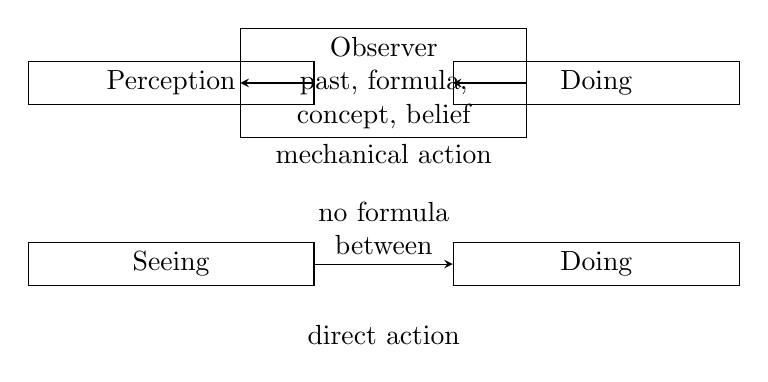
\begin{tikzpicture}[>=stealth]
\node[draw, align=center, text width=0.28\linewidth] (p1) at (-2.7,0) {Perception};
\node[draw, align=center, text width=0.28\linewidth] (o) at (0,0) {Observer\\past, formula,\\concept, belief};
\node[draw, align=center, text width=0.28\linewidth] (d1) at (2.7,0) {Doing};
\draw[->] (p1) -- (o);
\draw[->] (o) -- (d1);

\node[align=center] at (0,-0.9) {mechanical action};

\node[draw, align=center, text width=0.28\linewidth] (p2) at (-2.7,-2.3) {Seeing};
\node[draw, align=center, text width=0.28\linewidth] (d2) at (2.7,-2.3) {Doing};
\draw[->] (p2) -- node[above, align=center] {no formula\\between} (d2);

\node[align=center] at (0,-3.2) {direct action};
\end{tikzpicture}
\caption{Transcript-based reconstruction of the distinction between action through the observer and action as seeing-doing.}
\end{figure}

Krishnamurti's example is danger at the edge of a precipice. Seeing danger is instant action. One does not first construct an ideology of cliffs, derive a conclusion, and then act. The seeing is already the movement. He immediately adds that we are conditioned both to physical danger and to the idea that action requires a formula. The example is therefore not naive. It shows that direct action is intelligible, while also showing how deeply the mind is conditioned to mediation.

The last autobiographical example gives the same structure in a different register. A large spiritual organization had formed around Krishnamurti. In 1928 he saw that it was wrong, dissolved it, and returned the property. The importance of the example is not historical decoration. It shows the absence of regret when action does not arise from comparison, conclusion, or dependence. He saw and acted.

\section{Summary}

The lecture begins by questioning beauty as something stored in museums, art, poetry, cathedrals, and expert accounts. It then turns inward: beauty cannot be understood without passion, and passion is born when the mind does not withdraw from sorrow. This does not mean that suffering is to be cultivated. It means that escape from sorrow dissipates the energy needed to understand what is.

From there the inquiry widens into nature, sensitivity, conduct, and education. A civilization that becomes artificial, verbal, commercial, and linear loses contact not only with nature but with beauty in behaviour, speech, humility, and relationship. Education becomes suspect when it trains skill while neglecting fear, pleasure, relationship, order, beauty, and the whole field of life.

The final turn is action. Ordinary action follows idea, formula, pattern, memory, or ideology. Such action is mechanical because it is removed from perception. Krishnamurti's alternative is compressed in the phrase

\begin{equation}
\text{seeing} = \text{doing}.
\end{equation}

The chapter's conceptual spine is therefore not a doctrine of beauty but a sequence of distinctions: expression is not beauty; escape is not understanding; cultivated passion is not passion; education is not care; action according to idea is not free action. What remains is the possibility that, when the observer as past does not intervene, perception itself is action.